% !TEX root = ./main.tex
\documentclass[./main.tex]{subfiles}

\begin{document}
\chapter{Conclusion}

\section{Code statistics}

As counted by the \texttt{loc} \cite{loc} tool the project consist of \texttt{17,638} lines of code excluding
comments, black lines and library code.

\begin{figure}[H]
  \centering
  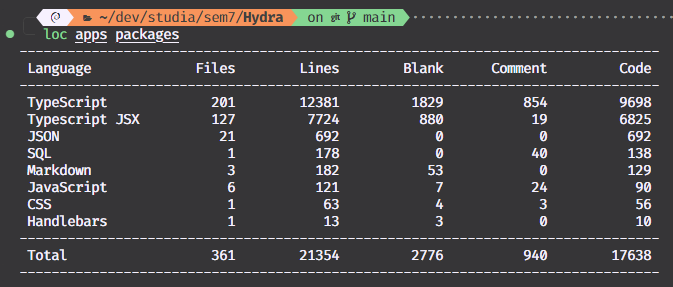
\includegraphics[width=0.8\textwidth]{code-stats.png}
  \caption{Lines of code divided by language}
\end{figure}

Full project code is available at \url{https://github.com/Critteros/Hydra} under the MIT license.

\section{Future development plans}

Future development plans include:

\begin{itemize}
  \item Adding more strategy templates for use. Including templates that support
        using boot menus
  \item Adding windows booting support
  \item Providing live monitoring of computers registered in the system
  \item Wake on LAN support
\end{itemize}


\section{Realization of the project goals}

All the functional requirements described in section \ref{subsec:functional-requirements} were implemented, and their
implementation was described in the implementation chapter \ref{chap:implementation}. As for the nonfunctional requirements, the system is secure and protects against SQL injection
attacks due to the use of ORM which eliminates the need of manually constructing
SQL queries.


Use of frontend framework protects against XSS attacks as the framework automatically escapes all the data that is rendered in the browser. The CRSF attacks are
not possible due to the same-site, secure cookie settings which prevents the browser
from sending them when a form is submitted from a different origin than the one
that set the cookie.

The performance of the system was not tested, but the system is designed to be
horizontally scalable, to handle more concurrent requests it is possible to add more
instances of the application server and load balance the requests between them.

Stored passwords are hashed using the bcrypt algorithm which is designed to
be slow and computationally expensive, this prevents brute-force attacks on the
password hashes. The schema for GraphQL API is publicly available and can be
used by external applications to interact with the system. Additionally all the data
exchange formats used by the system are standard and widely used, making it easy
to integrate with other systems.

The project can be considered a success as all the functional requirements were
implemented and the system is secure and performant. What is most important
is that the system is useful and can be used to manage booting of computers in a
network. Below figure shows test virtual machine booting SystemRescueCD from
the network using the boot system.

\begin{figure}[H]
  \centering
  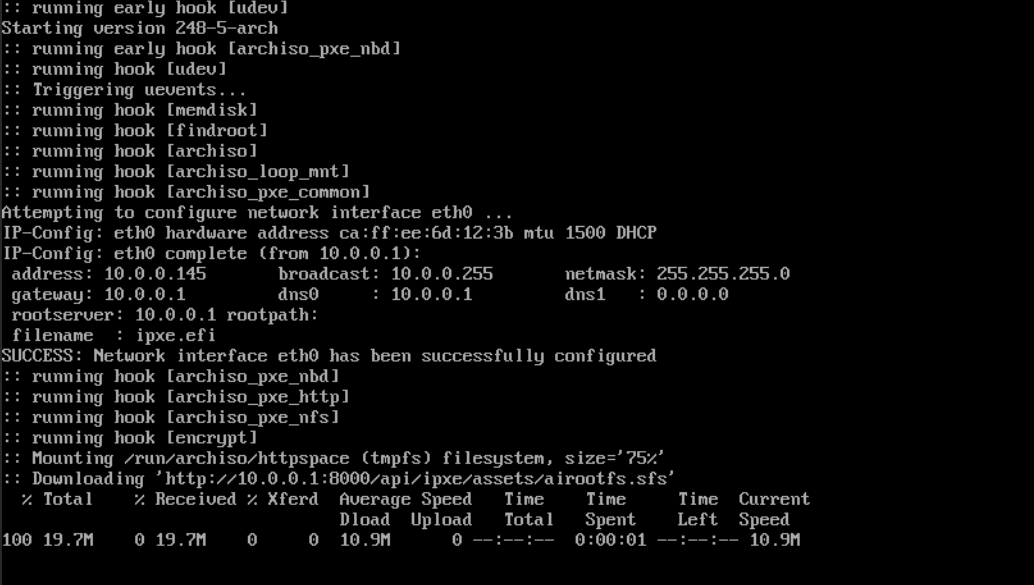
\includegraphics[width=\textwidth]{sysrescue-booting.png}
  \caption{SystemRescueCD booted from the network}
\end{figure}

\end{document}
